El diámetro de árbol se define como la longitud máxima que existe entre cualquier par de nodos que integren el árbol. Para poder calcular esta propiedad el árbol que se vaya analizar tiene que ser no dirigido y la aristas con un peso no negativo. Por ejemplo, considere el siguiente árbol:

% TODO: \usepackage{graphicx} required
\begin{figure}[h!]
	\centering
	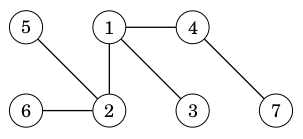
\includegraphics[width=0.5\linewidth]{img/diameter_tree_1}
	\label{fig:diametertree1}
\end{figure}

El diámetro de este árbol es 4, lo que corresponde al siguiente camino:

\begin{figure}[h!]
	\centering
	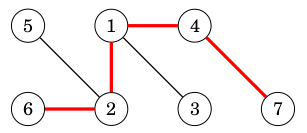
\includegraphics[width=0.5\linewidth]{img/diameter_tree_2}
	\label{fig:diametertree2}
\end{figure}

Tenga en cuenta que puede haber varias rutas de longitud máxima. En la ruta anterior, podríamos reemplazar el nodo 6 con el nodo 5 para obtener otra ruta con longitud 4. La siguiente guía va abordar como determinar el diámetro de un árbol.